% prelude.tex
%   - titlepage
%   - dedication (optional)
%   - approval sheet
%   - course certificate
%   - table of contents, list of tables and list of figures
%   - nomenclature
%   - abstract
%============================================================================


\clearpage\pagenumbering{roman}  % This makes the page numbers Roman (i, ii, etc)



% TITLE PAGE
%   - define \title{} \author{} \date{}
\title{Cryptanalysis of Round-Reduced \KECCAK{}}
\author{Nikhil Mittal}
\date{June, 2019}

%  - Roll number, required for the title page, approval sheet, and
%    certificate of course work 
\rollnum{17111056} 

%   - The default degree is ``Doctor of Philosophy''
%     (unless the document style msthesis is specified
%      and then the default degree is ``Master of Science'')
%     Degree can be changed using the command \iitbdegree{}
\iitbdegree{Master of Technology}

%   - The default report type is preliminary report.
%      * for a PhD thesis, specify \thesis
\thesis
%      * for a M.Tech./M.Phil./M.Des./M.S. dissertation, specify \dissertation
%\dissertation
%      * for a DIIT/B.Tech./M.Sc.project report, specify \project
%\project
%      * for any other type, use  \reporttype{}
%\reporttype{ReportType}

%   - The default department is ``Unknown Department''
%     The department can be changed using the command \department{}
\department{Computer Science \& Engineering}

%    - Set the guide's name
\setguide{Prof. Manindra Agrawal and Dr. Shashank Singh}
\setguidedept{Department of Computer Science \& Engineering}

%   - once the above are defined, use \maketitle to generate the titlepage
\maketitle

%--------------------------------------------------------------------%
\newpage
% CERTIFICATE
%     The first page after the title page.
%\makecertificate
% \includepdf[]{thesis-cert.pdf}

\includegraphics[width=\textwidth]{Selection_003.png}
\newpage
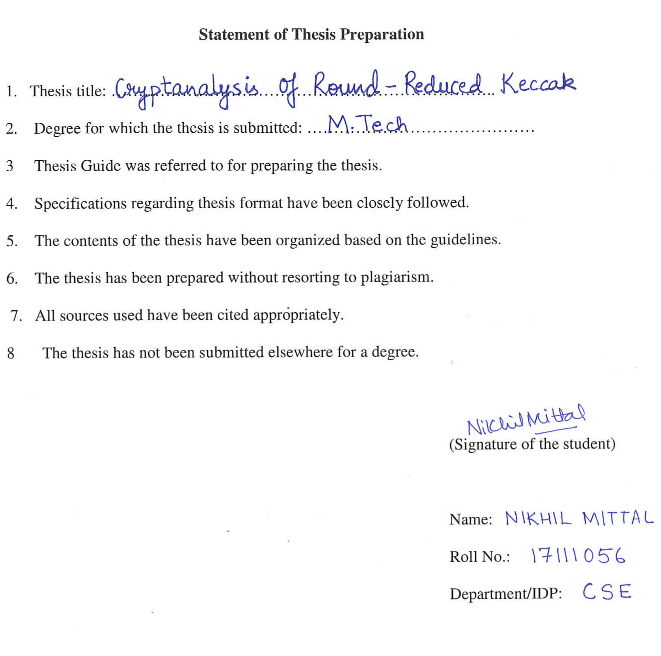
\includegraphics[width=\textwidth]{statement.png}
%------------------------------------------------------------------%
% COPYRIGHT PAGE
%   - To include a copyright page use \copyrightpage
% \copyrightpage

%--------------------------------------------------------------------%
% ABSTRACT
\begin{abstract}
	%The \KECCAK{} hash function is based on sponge construction which is different from previous \SHA{} standards. The \SHA-3 family of hash functions are based on \Keccak{}. \Keccak{}'s excellent resistance towards crypt-analytic attacks is one of the main reasons for its selection by NIST.
	
	In this thesis, we study the cryptanalysis of round reduced variants of
	\KECCAK{} hash function. The \KECCAK{} hash function is based on sponge
	construction which is different from previous \SHA{} standards. 
	\KECCAK{} faced a lot of cryptanalysis since it was declared as the
	winner of the \SHA-3 contest. The techniques such as computing partial
	solutions,  linearization etc. are used for the cryptanalysis of
	round-reduced \KECCAK{}. These techniques are very effective for
	mounting preimage attacks on $2$ to $3$ rounds of round-reduced \KECCAK{}. 
	
	The main contribution of the thesis is a cryptanalysis of $2$ rounds of 
	round reduced
	\KECCAK{}$[r:=800-384, c:=384]$. 
	The best-known preimage
	attack for this variant of \KECCAK{} has the time complexity of
	$O(2^{64})$. We propose a preimage attack with an improved time and
	space complexity of $O(2^{44})$. We further analyze the linear structure
	technique provided by Guo \etal and suggested preimage attacks for $3$ rounds of \KECCAK-$256$ and $4$ rounds of \KECCAK-$224$.
\end{abstract}

%--------------------------------------------------------------------%
% DEDICATION
%   Dedications, if any.
\begin{dedication}
	To my family
\end{dedication}

% Acknowledgements
\begin{acknowledgments}
	
	I would like to thank all the people who helped me during my thesis. I thank my thesis co-supervisor \textbf{Dr. Shashank Singh} for his guidance and motivating me to keep trying.
	My sincere thanks to my thesis co-supervisor \textbf{Prof. Manindra Agrawal}, who readily agreed to co-supervise me after Dr. Shashank Singh moved to IISER Bhopal. 
	% 
	% I also thank the reviewers of Indocrypt-$2018$ for providing comments which helped in improving the work. In particular, we thank an anonymous reviewer for suggesting us to implement the attack on the $\Keccak[r:=400-192,\, c:=192]$ and also providing insights to further improve the attack. 
	% 
	I would also like to thank Rajendra Kumar and Mahesh Sreekumar Rajasree
	for their valuable time, discussions, and guiding me in every possible
	way. I thank all the faculty members of department of computer science
	and engineering (CSE), IIT Kanpur who taught me during the course of my
	MTech degree. I have learned a lot from their teachings. A special
	thanks to the CSE department for providing all the facilities that were required and  IIT Kanpur for my academic as well as personal growth.
\end{acknowledgments}

%--------------------------------------------------------------------%
% CONTENTS, TABLES, FIGURES
\tableofcontents
\listoftables

\cleardoublepage
\phantomsection \label{listoffig}
\listoffigures

\cleardoublepage\pagenumbering{arabic} % Make the page numbers Arabic (1, 2, etc)
